\subsection{树、森林和二叉树的转换}

\subsubsection{树转换为二叉树}
\begin{frame}\ft{\subsubsecname}
  将树转换为二叉树的步骤:
  \begin{itemize}
  \item[1.]  \blue{加线:}在所有兄弟节点之间加一条连线。\\[0.1in]
  \item[2.]  \blue{去线:}对树中每个结点,只保留它和第一个孩子结点的连线,删除它与其他孩子结点之间的连线。\\[0.1in] 
  \item[3.]  \blue{层次调整:}以树的根结点为轴心,将整棵树顺时针旋转一定角度,使之结构层次分明。注意第一个孩子是二叉树结点的左孩子,兄弟转换过来的孩子是结点的右孩子。
  \end{itemize}
\end{frame}


\begin{frame}\ft{\subsubsecname}
  \begin{figure}
    \centering
    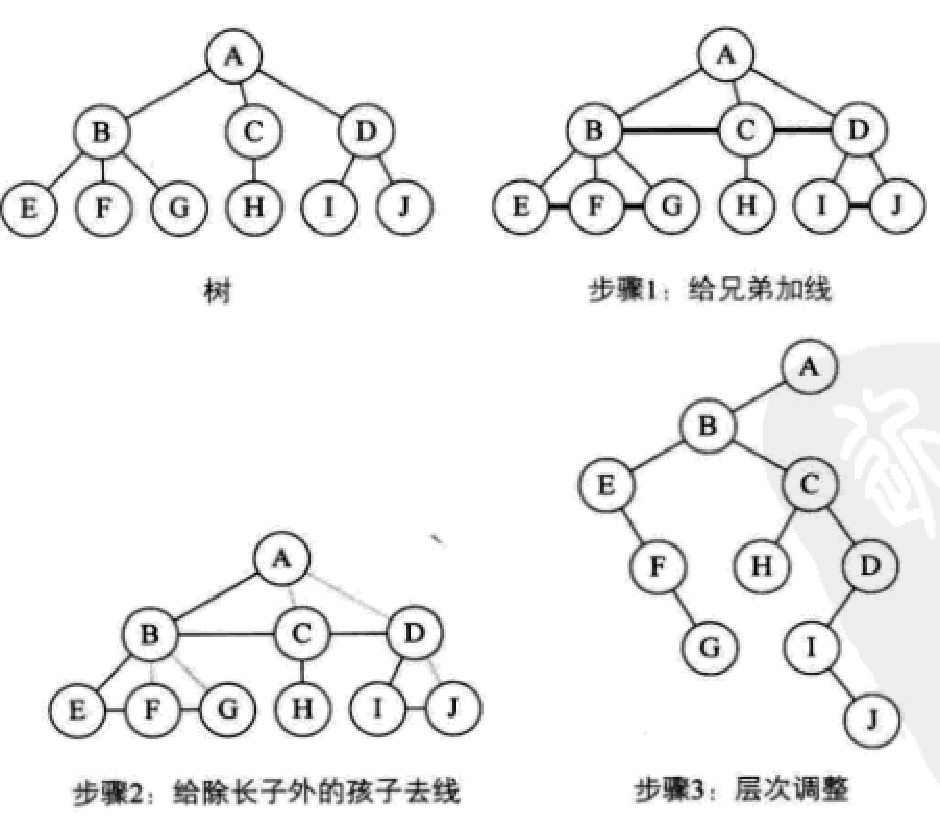
\includegraphics[width=3.5in]{Chapters/Ch05/Fig/tree2bitree.pdf}
  \end{figure}
\end{frame}

\subsubsection{森林转换为二叉树}
\begin{frame}\ft{\subsubsecname}
  步骤:
  \begin{itemize}
  \item[1.]  把每棵树转换为二叉树。\\[0.1in]
  \item[2.]  第一棵二叉树不动,从第二棵二叉树开始,依次把后一棵二叉树的根结点作为前一棵二叉树的根结点的右孩子,用线连接起来。当所有的二叉树连接起来后就得到了由森林转换来的二叉树。
  \end{itemize}
\end{frame}

\begin{frame}\ft{\subsubsecname}
  \begin{figure}
    \centering
    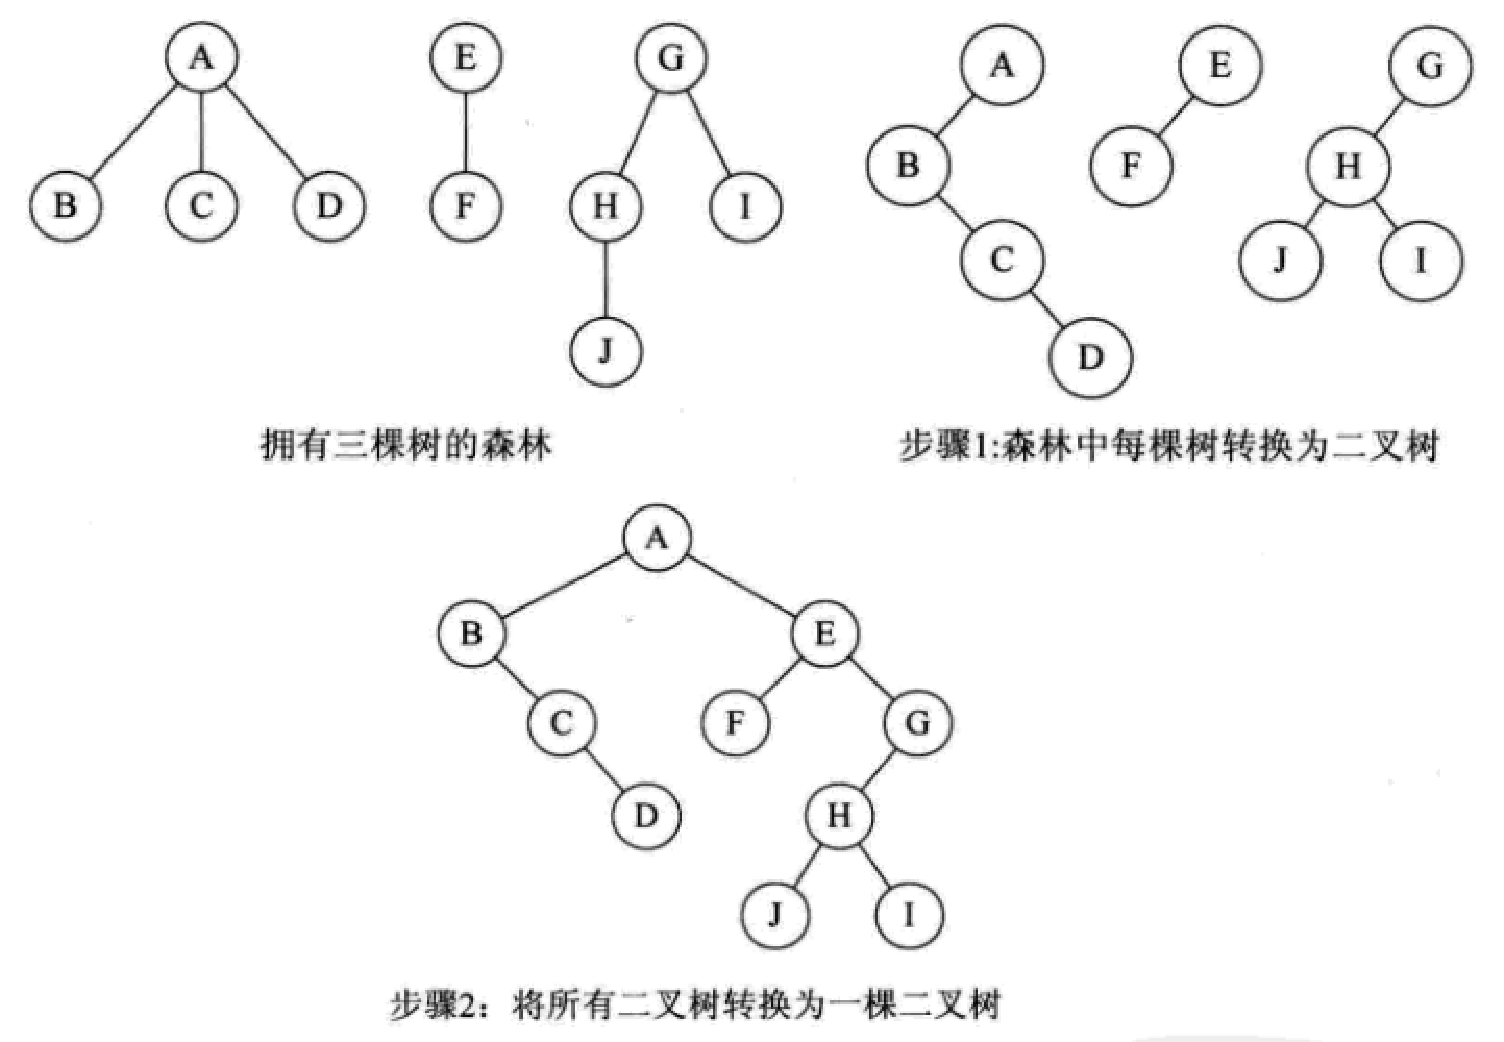
\includegraphics[width=4in]{Chapters/Ch05/Fig/forest2bitree.pdf}
  \end{figure}
\end{frame}


\subsubsection{二叉树转换为树}
\begin{frame}\ft{\subsubsecname}
  步骤:
  \begin{itemize}
  \item[1.]  \blue{加线:}若某结点的左孩子存在,则将这个左孩子的右孩子、右孩子的右孩子、右孩子的右孩子的右孩子、......,即左孩子的$n$个右孩子作为此结点的孩子。将该结点与这些右孩子用线连接起来。\\[0.1in]
  \item[2.]  \blue{去线:}删除原二叉树中所有结点与其右孩子的连线。\\[0.1in] 
  \item[3.]  \blue{层次调整:}使之结构层次分明。
  \end{itemize}
\end{frame}

\begin{frame}\ft{\subsubsecname}
  \begin{figure}
    \centering
    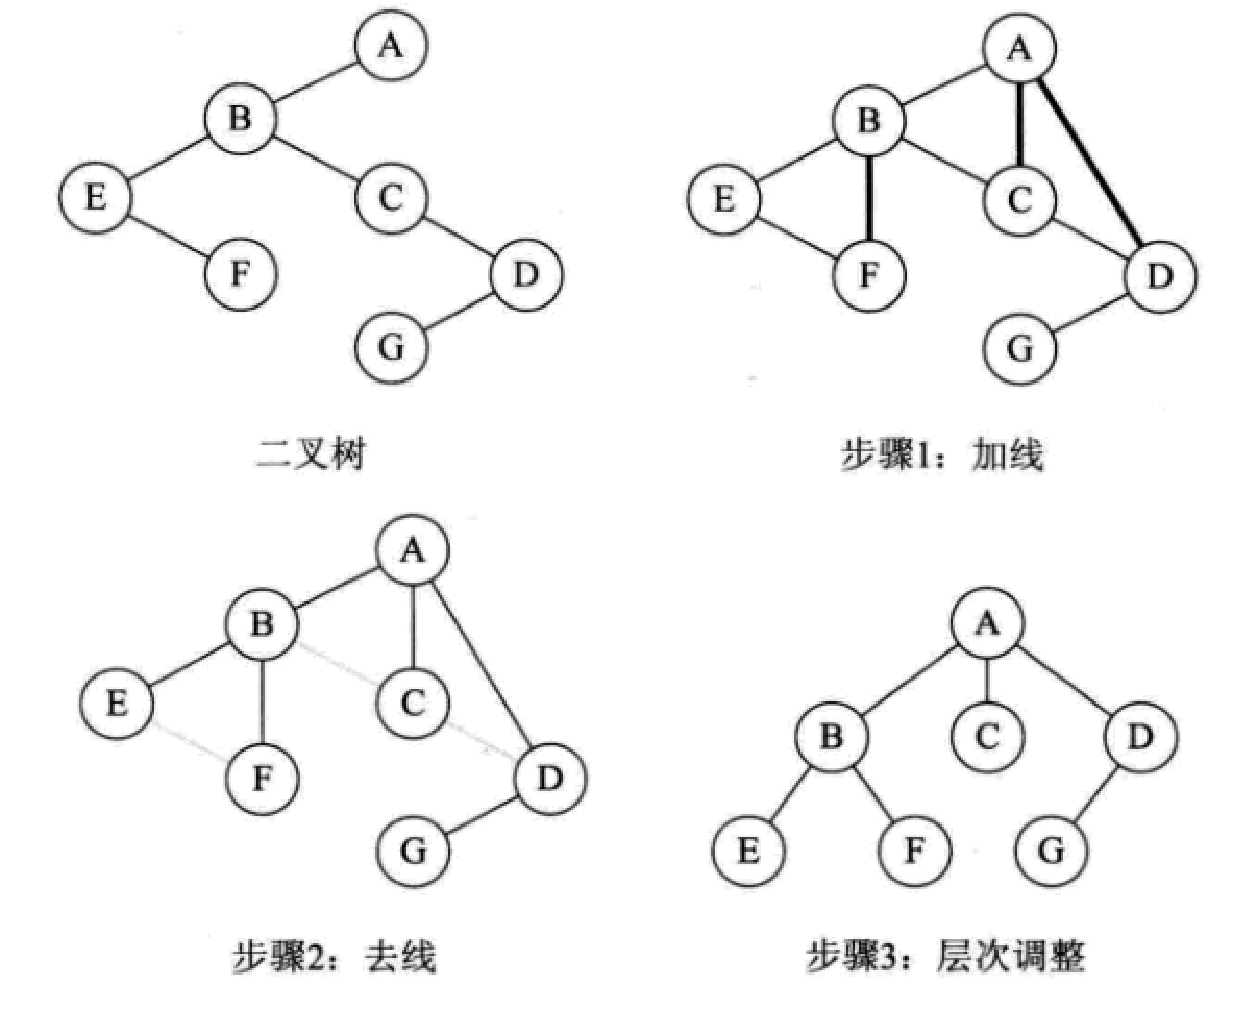
\includegraphics[width=4in]{Chapters/Ch05/Fig/bitree2tree.pdf}
  \end{figure}
\end{frame}

\subsubsection{二叉树转换为森林}
\begin{frame}\ft{\subsubsecname}
  判断一棵二叉树能够转换成一棵树还是森林,只要看这棵二叉树的根结点有没有右孩子,有就是森林,没有就是一棵树。转换成森林的步骤:
  \begin{itemize}
  \item[1.] 从根结点开始,若右孩子存在,则把与右孩子结点的连线删除,再查看分离后的二叉树,若右孩子存在,则连线删除,......,直到所有右孩子连线都删除为止,得到分离的二叉树。\\[0.1in]
  \item[2.] 再将每棵分离后的二叉树转换为树即可。
  \end{itemize}
\end{frame}

\begin{frame}\ft{\subsubsecname}
  \begin{figure}
    \centering
    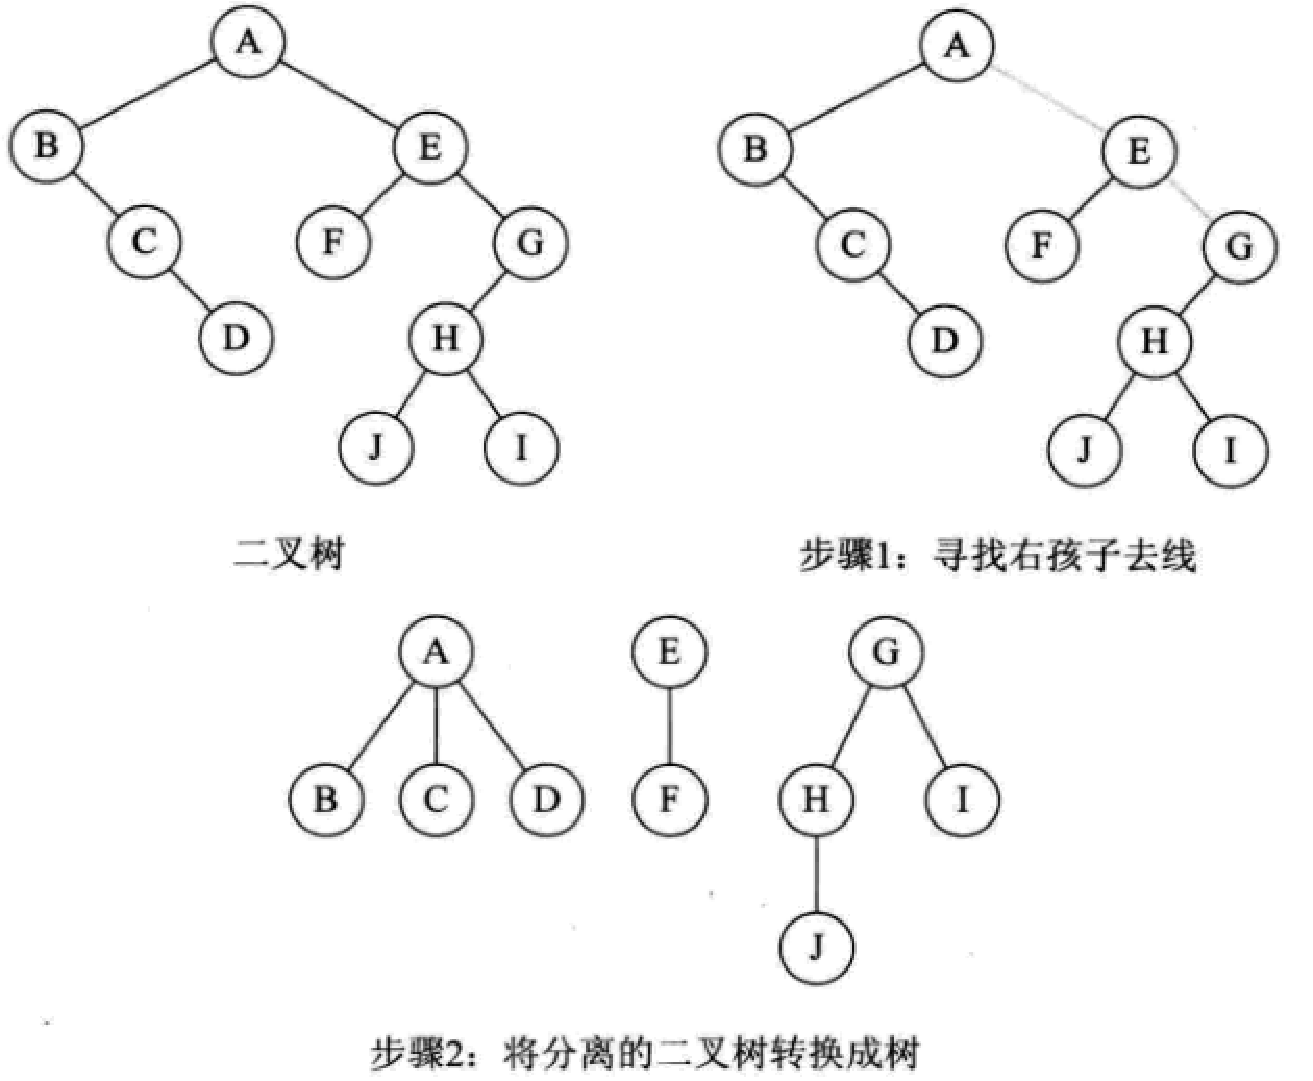
\includegraphics[width=4in]{Chapters/Ch05/Fig/bitree2forest.pdf}
  \end{figure}
\end{frame}

\subsubsection{树和森林的遍历}
\begin{frame}\ft{\subsubsecname}
  树的遍历分为两种方式:
  \begin{itemize}
  \item[1.] \blue{先根遍历:}先访问树的根结点,然后依次先根遍历根的每棵子树。
  \item[2.] \blue{后根遍历:}先依次后根遍历每棵子树,然后再访问根结点。
  \end{itemize}

  %\pause 
  \begin{figure}
    \centering
    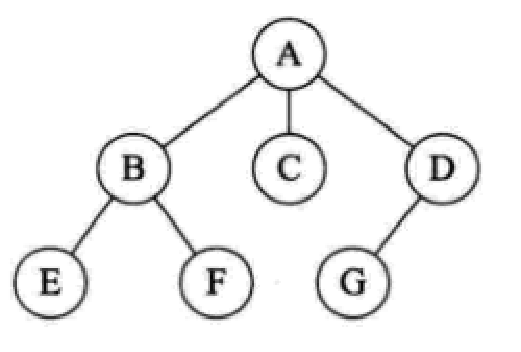
\includegraphics[width=1.8in]{Chapters/Ch05/Fig/tree.pdf}
  \end{figure}

  %\pause 
  \tf先根遍历序列为A、B、E、F、C、D、G;

  \tf后根遍历序列为E、F、B、C、G、D、A。
\end{frame}

\begin{frame}\ft{\subsubsecname}
  森林的遍历也分为两种方式:
  \begin{itemize}
  \item[1.] \blue{前序遍历:}先访问森林中第一棵树的根结点,然后再依次先跟遍历根的每棵子树,再依次用同样方式遍历除去第一棵树的剩余树构成的森林。
  \item[2.] \blue{后序遍历:}先访问森林中第一棵树,后根遍历每棵子树,然后再访问根结点,再依次同样方式遍历除去第一棵树的剩余树构成的森林。
  \end{itemize}

  %\pause 
  \begin{figure}
    \centering
    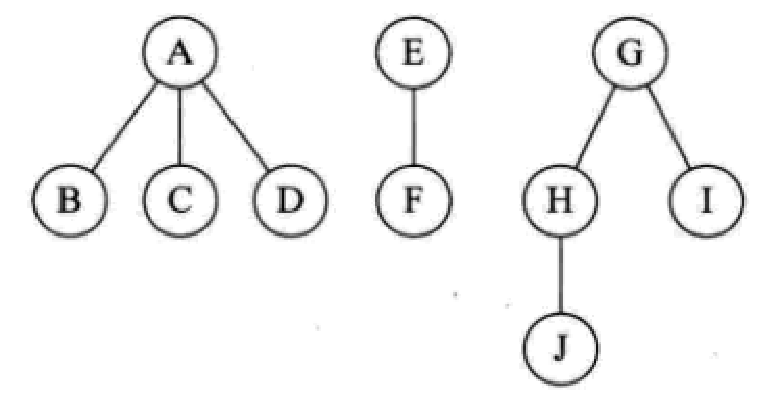
\includegraphics[width=2.5in]{Chapters/Ch05/Fig/forest.pdf}
  \end{figure}

  %\pause 
  \tf先根遍历序列为A、B、C、D、E、F、G、H、J、I;

  \tf后根遍历序列为B、C、D、A、F、E、J、H、G。
\end{frame}

\begin{frame}\ft{\subsubsecname}
  \begin{figure}
    \centering
    \begin{minipage}{0.45\textwidth}
      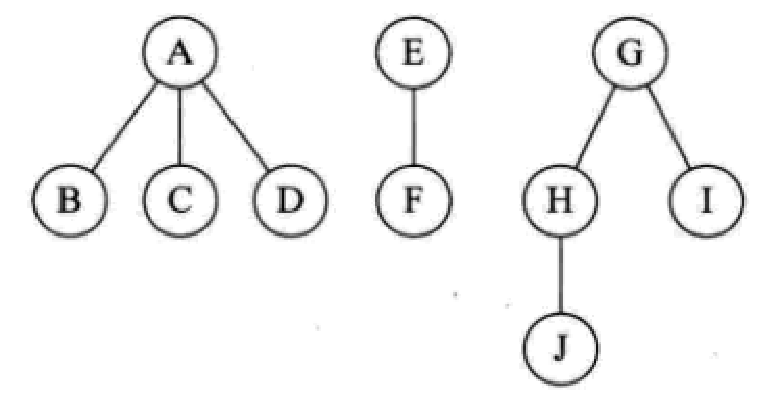
\includegraphics[width=2.2in]{Chapters/Ch05/Fig/forest.pdf}  
    \end{minipage}
    \begin{minipage}{0.45\textwidth}
      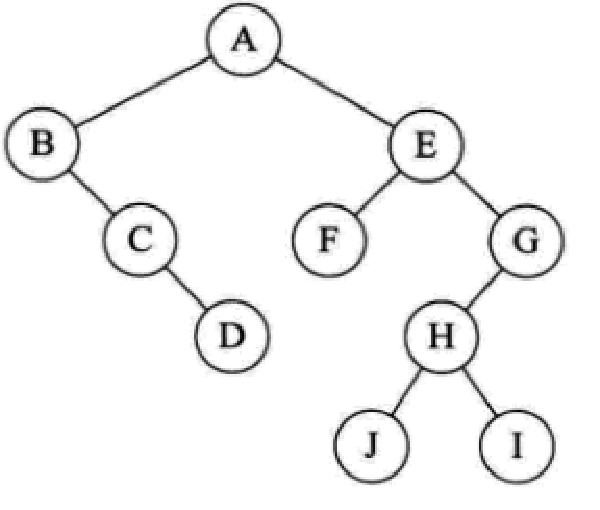
\includegraphics[width=1.6in]{Chapters/Ch05/Fig/bitree.pdf}  
    \end{minipage}    
  \end{figure}
  %\pause 
  \blue{森林的前序遍历和二叉树的前序遍历结果相同,森林的后续遍历和二叉树的中序遍历结果相同。}
\end{frame}
